\documentclass{article}

\usepackage[margin=1.6cm]{geometry}
\usepackage{amsmath,amssymb}
\usepackage{float}
\usepackage{graphicx}
\usepackage{fancyhdr}
\pagestyle{fancy}
\usepackage{tcolorbox,listings}
\usepackage{color}
\usepackage{hyperref}
\renewcommand\headrulewidth{1pt}
\usepackage{marvosym}
\usepackage{xcolor}
\usepackage{tikz}
%\usepackage{babel}
\usepackage[french]{babel}
\usepackage[babel=true,kerning=true]{microtype}
\usepackage{afterpage}

\newcommand\myemptypage{
    \null
    \thispagestyle{empty}
    \addtocounter{page}{-1}
    \newpage
    }

\usetikzlibrary{
  arrows,
  calc,
  shapes.geometric,
  shapes.misc,
  shapes.symbols,
  shapes.arrows,
  automata,
  through,
  positioning,
  scopes,
  decorations.shapes,
  decorations.text,
  decorations.pathmorphing,
  shadows}

\definecolor{darkWhite}{rgb}{0.94,0.94,0.94}
 
\lstset{
    backgroundcolor=\color{darkWhite},
    breakatwhitespace=false,
    breaklines=true,
    captionpos=b,
    commentstyle=\color{green},
    deletekeywords={...},
    escapeinside={\%*}{*)},
    extendedchars=true,
    keepspaces=true,
    keywordstyle=\color{blue},
    %language=Python,
    morekeywords={*,...},
    showspaces=false,
    showstringspaces=false,
    showtabs=false,
    stepnumber=1,
    stringstyle=\color{gray},
    tabsize=4,
}
 
\lstdefinestyle{frameStyle}{
    basicstyle=\sffamily,
    numbers=left,
    numbersep=20pt,
    numberstyle=\tiny\color{black}
}
 
\tcbuselibrary{listings,skins,breakable}
 
\newtcblisting{customFrame}{
    arc=0mm,
    top=0mm,
    bottom=0mm,
    left=3mm,
    right=0mm,
    width=\textwidth,
    listing only,
    listing options={style=frameStyle},
    breakable
}

\fancyhead[L]{ALLEMAND Fabien\\??? Samuel}
\fancyhead[C]{Systèmes Complexes et Optimisation Stochastique Massivement Parallèle}
\fancyhead[R]{
\includegraphics[scale=0.08]{img/logo_UFR_1.png}}
\fancyfoot[L]{Rapport de Projet}
\fancyfoot[R]{\today}

\begin{document}

\newpage
\thispagestyle{empty}
\addtocounter{page}{-1}
\begin{center}
	\baselineskip=50pt
	\vspace*{1cm}
	\textbf{{\Huge Systèmes Complexes et Optimisation Stochastique Massivement Parallèle}}\\
	\vspace*{0.25cm}
	\textbf{{\Huge Rapport de Projet}}\\
	\vspace*{0.25cm}
	\begin{minipage}[c]{.46\linewidth}
        \centering
        \textbf{Equipe:}\\
		ALLEMAND Fabien\\
        ??? Samuel
    \end{minipage}
\end{center}
\vspace{0.1cm}

\begin{figure}[H]
\centering
\centerline{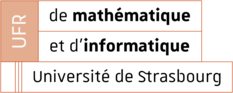
\includegraphics[scale=1.]{img/logo_UFR_2.png}}
\end{figure}

\newpage
\myemptypage

% \pagenumbering{roman}

% \newpage
% \myemptypage

\newpage
% \addcontentsline{toc}{section}{Table des matières}
\renewcommand{\contentsname}{Table des matières}
\tableofcontents

\newpage
\addcontentsline{toc}{section}{Liste des figures}
\renewcommand{\listfigurename}{Liste des figures}
\listoffigures

\pagenumbering{arabic}

\newpage
\section{Introduction}
Evolutionary algorithms and genetic programming are used in a wide range of
applications. From basic applications in industry and engineering to complex
problem resolution in resarch department, these two methods, whose development
started with Alan Turing in 1950, no longer need to prove their efficiency.\\

% State of the art?

On the one hand, evolutionary algorithms, inspired by biological evolution,
allows us to find quatities or caracteristics of an object, and on the other
hand, genetic programming was designed to find interactions between objects. By
combining these two methods, it is theoredicaly possible (assuming there is a
good way to evaluate our results) to find not only caracteritics defining two
entities, but also the way they interact with each other.
These two entities could very well be daily life objects or even animals. We
could actually be able to find how birds interact with each other in a flock.
These two entites could be less concrete and be ridiculously small: let us find
out how electrons interact in matter! But they could also be enormous like
celestial bodies...\\

Let us go back in time and imagine we only have the knowledge and tools to
measure the position of the Sun relatively to the Earth. Would we be able to
find caracteritics about the Earth or the Sun like their mass or their speed?
Is there a way to find out how they interact?\\

The goal of this project is to utilise the two afore mentionned programming
methods to retrieve caracteristics and laws regarding the interactions between
two celestial bodies.\\
We will focus on Earth and Sun as there is a strong interaction between them
and yet are comletely different.\\
First, we will conduct a physics study regarding the celestial bodies in order
to evaluate results to come.
In a second time, we will attempt to find caracteristics about the two planets using
evolutionary algorithms. Finally, we will use genetic programming to
re-discover Newton's law
of universal gravitation.

% Try with another planet as an exemple of generality~
% Use multi-thread/core and compare perfomrance ?

\newpage
\section{Conclusion}

In conclusion, we first used evolutionary algorithms to find the mass of the
earth, the mass of the sun and the speed at which the earth revolves around the
sun. EA proved to be able to solve these problems without any issue and in a
short time.\\
The second part of the project was dedicated to the recovery of Newton's
universal law of gravitation. However, during this part, Easena prevented us
from implementing our solution as we wanted. We then had to improvise and use a
different approach to solve the problem. This approach was successful, but it
was not as effective as we had originally planned. Nevertheless, we were able
to complete the project and obtain valuable information about the process, such
as the influence of the parameter on the convergence speed and the quality of
the final results.\\

Now that we know that genetic programming is capable of finding a physical law
from simple observations and constants, it would be interesting to see if GP is
also capable of finding more complex models such as the Navet-Stokes equations,
which describe fluid flow, perhaps by taking advantage of the acceleration
offered by island parallelism with GPGPU.\\

\newpage
\addcontentsline{toc}{section}{Bibliographie}
\renewcommand{\refname}{Bibliographie}
\bibliographystyle{plain}
\bibliography{bibliographie}

\newpage
\myemptypage

\newpage
\input{src/annexes.tex}

\end{document}